\chapter{Projekt- und Qualitätsmanagement}
	\label{cap:projectmanagement}
	
	Zur Verwaltung des Projektes hat das Projektteam ein Jira eingesetzt.
	
	\section{Projektmanagement}
		Zur Grobplanung und zur Planung der Meilensteine wurden Jira-Versions eingesetzt.
		Die Meilensteine hat das Projektteam zu Beginn des Projekts definiert und zeitlich festgelegt.
		Diese Planung ist auch in Abbildung~\ref{fig:jiraVersions} zu sehen.
		
		Für die Architektur-Meilensteine und die Meilensteine zum Abschluss der Dokumentation wurde bereits bei der Grobplanung deren Inhalt entschieden.
		Für die Entwicklungsmeilensteine wurde, wie im agilen Projektmanagement üblich,
		deren Inhalt jeweils zu Beginn zusammen mit dem Betreuer als Ansprechpartner der Kundengruppe definiert.
		
		\begin{figure}[H]
			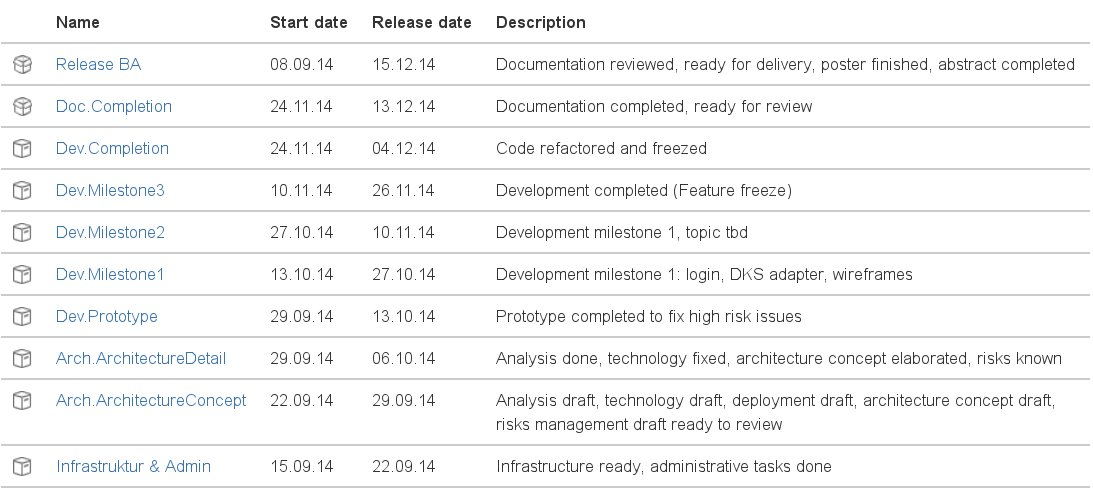
\includegraphics[width=\textwidth]{projectPlan/media/img/jiraVersions.jpg}
			\centering
			\caption{Projektplan (Jira Versions/Meilensteine)}
			\label{fig:jiraVersions}
		\end{figure}
		
		Features haben wir in Zusammenarbeit mit dem Vertreter der Kundengruppe priorisiert und daraus resultierende Issues Meilensteine zugeordnet.
		Zur Strukturierung haben wir zusätzlich Labels eingesetzt.
		
		\begin{figure}[H]
			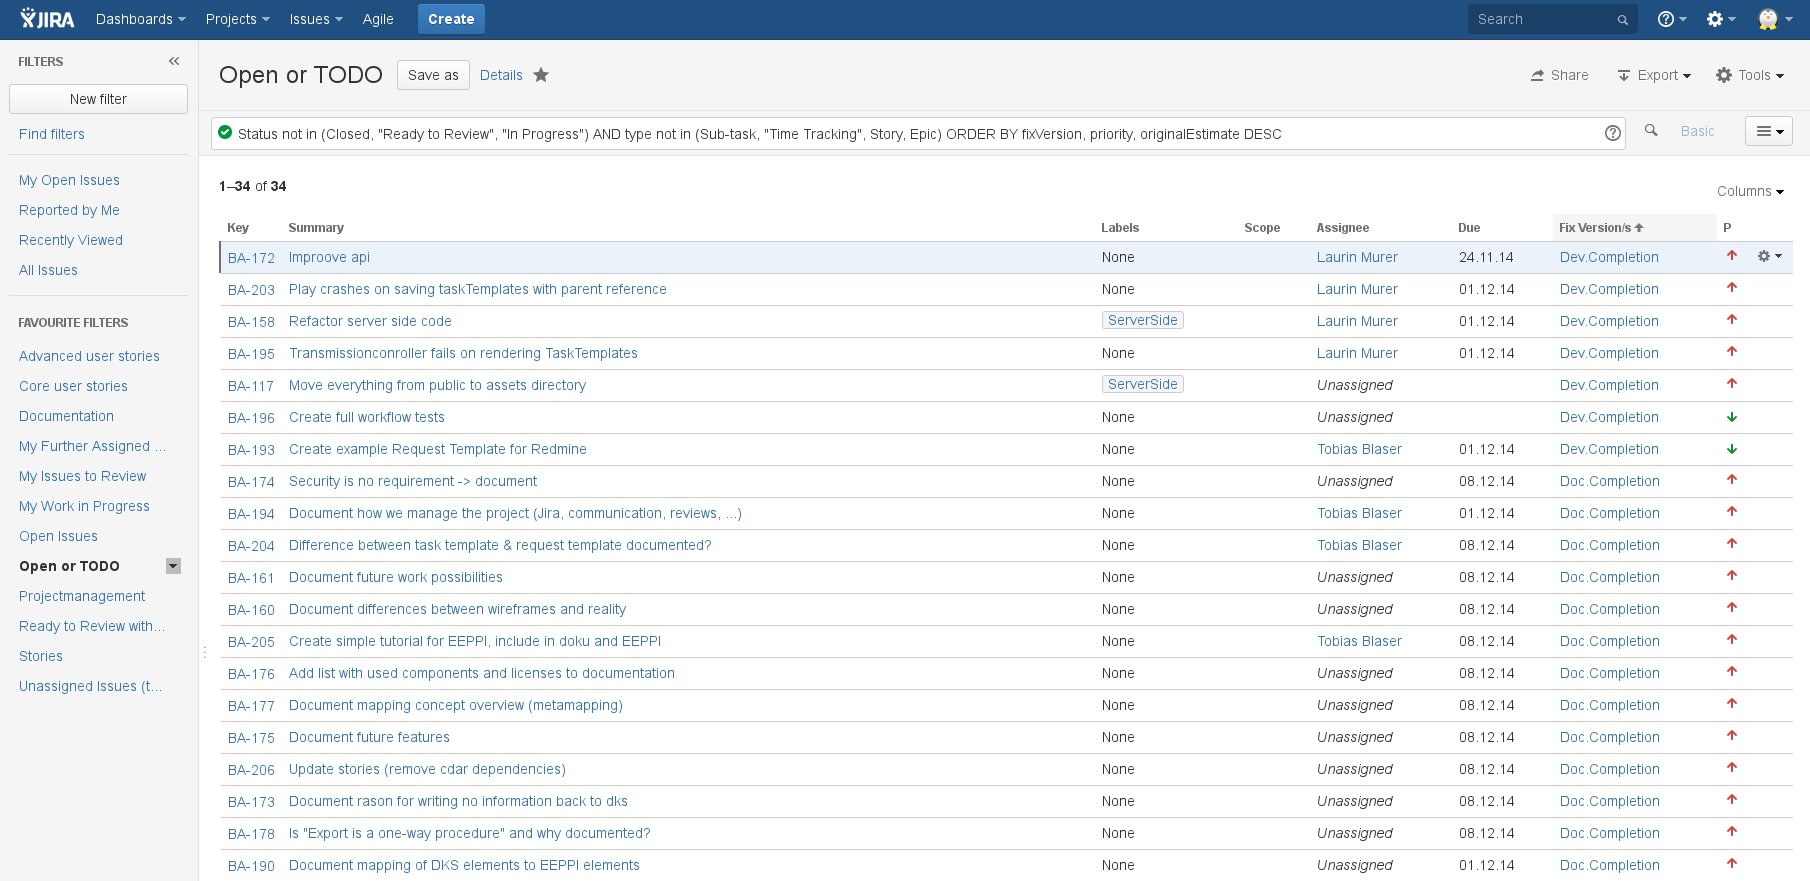
\includegraphics[width=\textwidth]{projectPlan/media/img/jiraIssuesOpenOrTodo.jpg}
			\centering
			\caption{Beispiele von Jira Issues, sortiert nach Version}
			\label{fig:jiraIssuesOpenOrTodo}
		\end{figure}
		
		Anhand den geschätzten Aufwänden
		pro Issue und der zur Verfügung stehenden Zeit eines Meilensteine haben wir jeweils eine Meilensteinplanung durchgeführt.		
		Dabei haben wir maximal 2/3 der zur Verfügung stehenden Zeit für
		Issues eingeplant und den Rest für Unvorhergesehenes, 
		Meetings und Planung vorgesehen.
		
		\begin{figure}[H]
			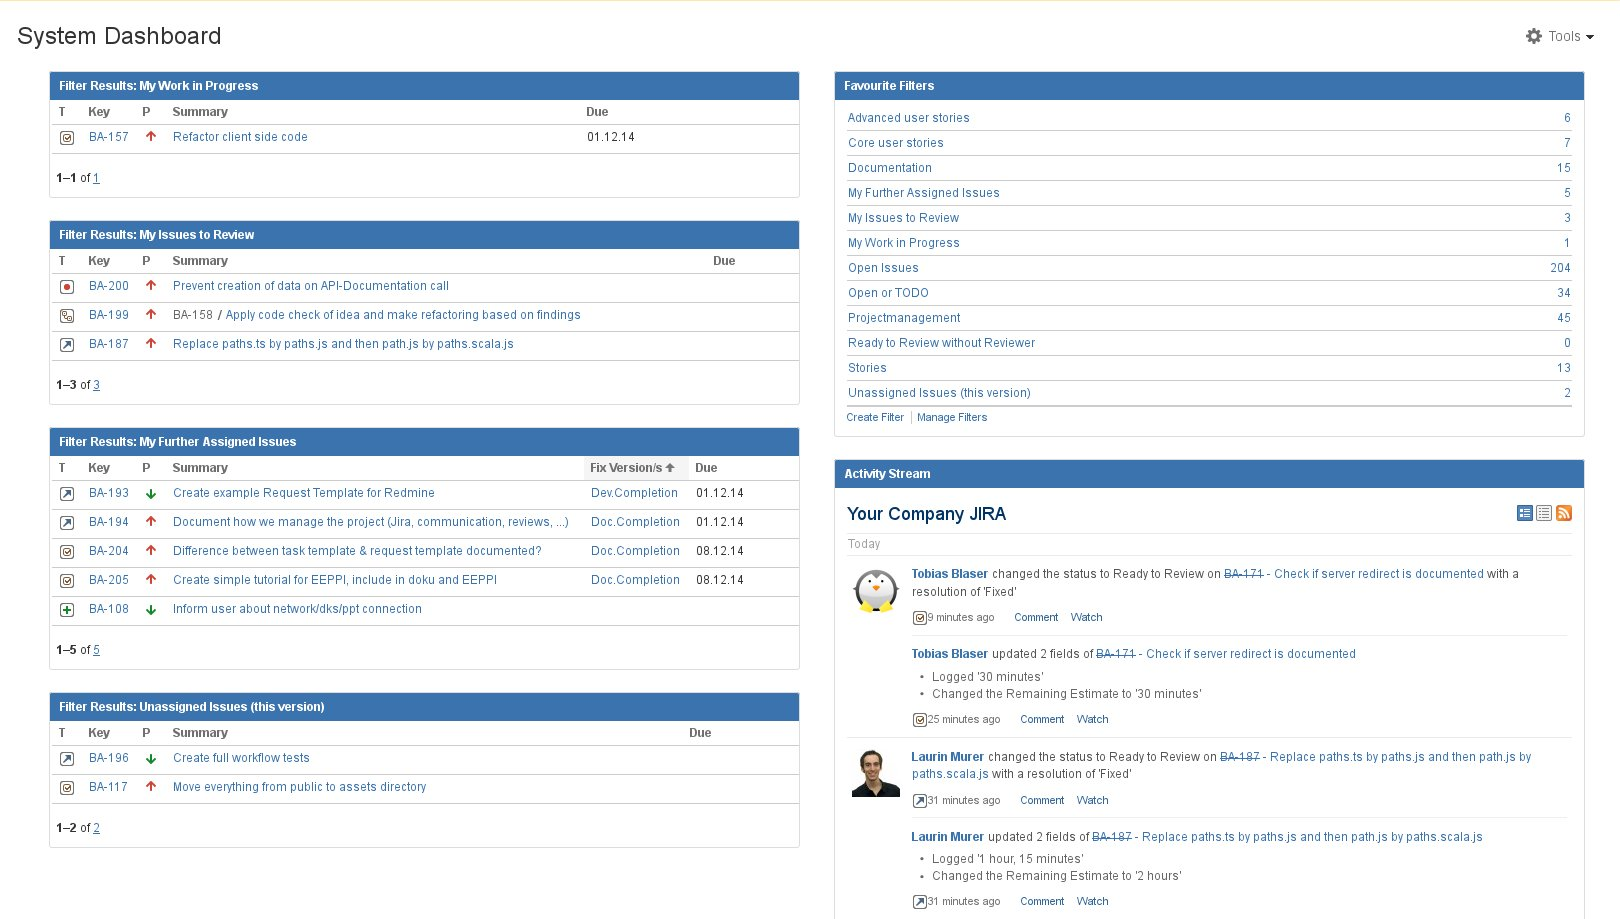
\includegraphics[width=\textwidth]{projectPlan/media/img/jiraDashBoard.jpg}
			\centering
			\caption{Jira Dashboard Beispiel}
			\label{fig:jiraDashBoard}
		\end{figure}
		
		Jira bietet anpassbare Dashboards, 
		die einen Überblick über das laufende Projekt bieten.
		
		Der Activity Stream von Jira sowie die Git History ermöglichten es uns auf einfache Weise nachzuvollziehen,
		an was der Teampartner in den letzten Stunden gearbeitet hat. 
		Dies senkt den Kommunikationsaufwand und die Notwendigkeit,
		jederzeit gemeinsam an einem Ort zu arbeiten.
		
		\begin{figure}[H]
			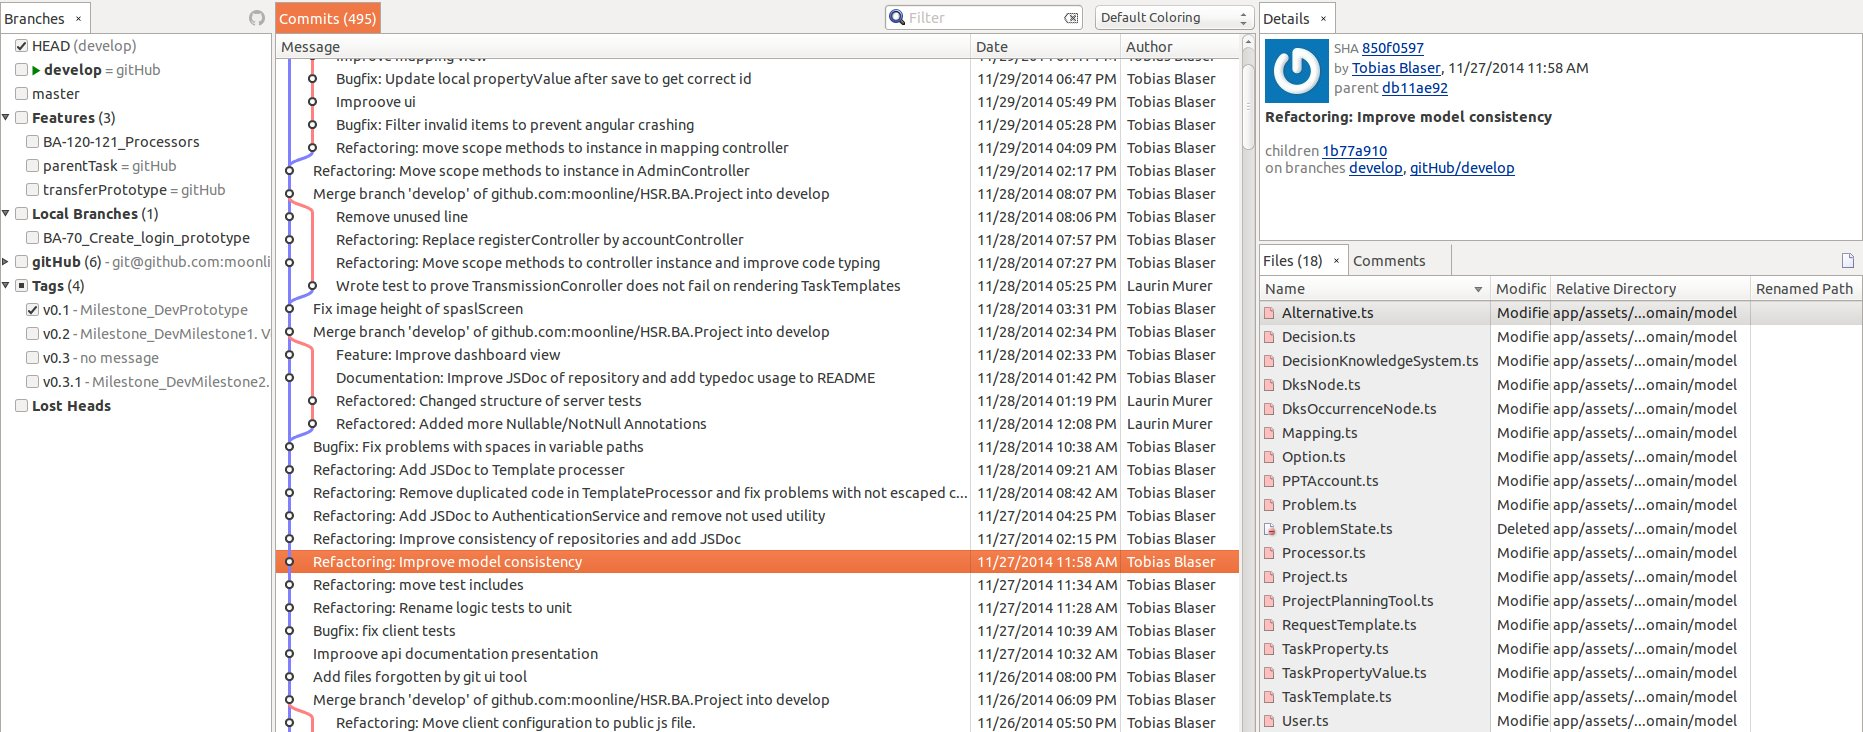
\includegraphics[width=\textwidth]{projectPlan/media/img/gitHistory.jpg}
			\centering
			\caption{Git History in SmartGit}
			\label{fig:gitHistory}
		\end{figure}
		
		Für grössere Features haben wir Git Flow Featurebranches eingesetzt.
		Für Releases entsprechend Releasebranches.
		Zusätzliche haben wir die Funktion "<Releases"> von Github
		zum Hinzufügen von fertigen Builds zu Releases genutzt.
		
		\begin{figure}[H]
			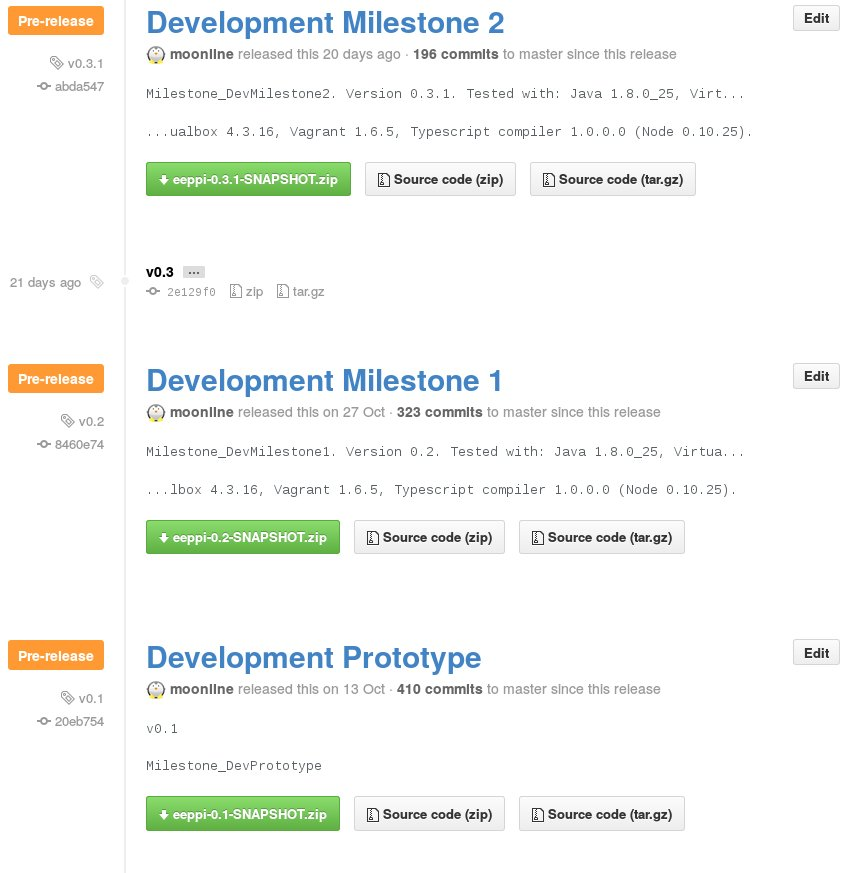
\includegraphics[width=0.5\textwidth]{projectPlan/media/img/githubReleases.jpg}
			\centering
			\caption{Github Releases mit Build-Archives}
			\label{fig:githubReleases}
		\end{figure}
	
		
	\section{Qualitätssicherung}
		Um sicherzustellen, dass keine Issues geschlossen werden,
		ohne dass die Arbeit einem Review unterzogen wurde,
		haben wir den Issue Workflow im Jira entsprechend gestaltet.		
		
		\begin{figure}[H]
			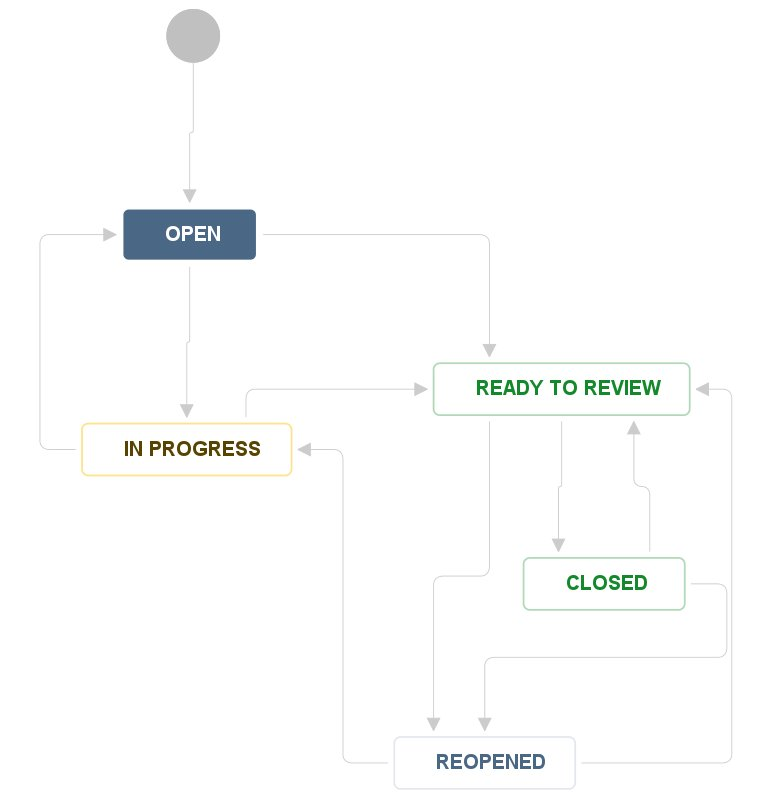
\includegraphics[width=0.5\textwidth]{projectPlan/media/img/jiraIssueWorkflow.jpg}
			\centering
			\caption{Angepassten Jira Issue-Workflow}
			\label{fig:jiraIssueWorkflow}
		\end{figure}
		
		Fertig gestellte Issues müssen immer dem andern Teammitglied
		zum Review gesandt werden und tauchen entsprechend auf dessen
		Dashboard als "<Ready to Review"> auf.
		
		Es geht dabei nicht darum, 
		für jeden erledigten Issue den kompletten Code des Andern anzusehen, 
		sondern das Resultat grob anzuschauen und eventuell
		Edge-Cases\footnote{Spezialfälle, bezogen auf Input Daten oder 
		Workflows der grafischen Oberfläche} zu prüfen. 
		Ein komplettes Code Review jedes Issues wäre zeitlich nicht verhältnismässig.
		
		
		\section{Testkonzept}
			\label{sec:testkonzept}
		
			Um zuverlässig alle notwenigen Bereiche mit Tests abzudecken, 
			werden folgende Tests durchgeführt:
			
			\begin{description}
				\item[Unit (Unit- /Logiktests)] Tests, die eine einzelne Klasse, 
					Service oder Komponente testen. 
					Andere Klassen sind nur soweit Teil des Tests, 
					wie dies aufgrund der Abhängigkeiten notwendig ist.
					\begin{figure}[H]
						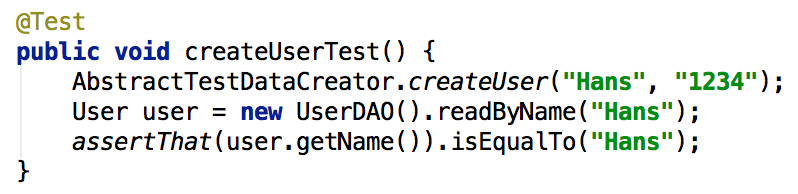
\includegraphics[scale=0.5]{projectPlan/media/img/unitTest.png}
						\centering
						\caption{Beispiel eines Unittests}
						\label{fig:exampleUnittest}
					\end{figure}

				\item[Integration (Integrationstests)] Tests, die das Zusammenspiel zwischen Klassen, 
					Komponenten und Services testen. 
					Diese Tests können über mehrere Layers bis mehrere Tiers laufen.
					Alle API-Aufrufe werden mit solchen Tests getestet.
					\begin{figure}[H]
						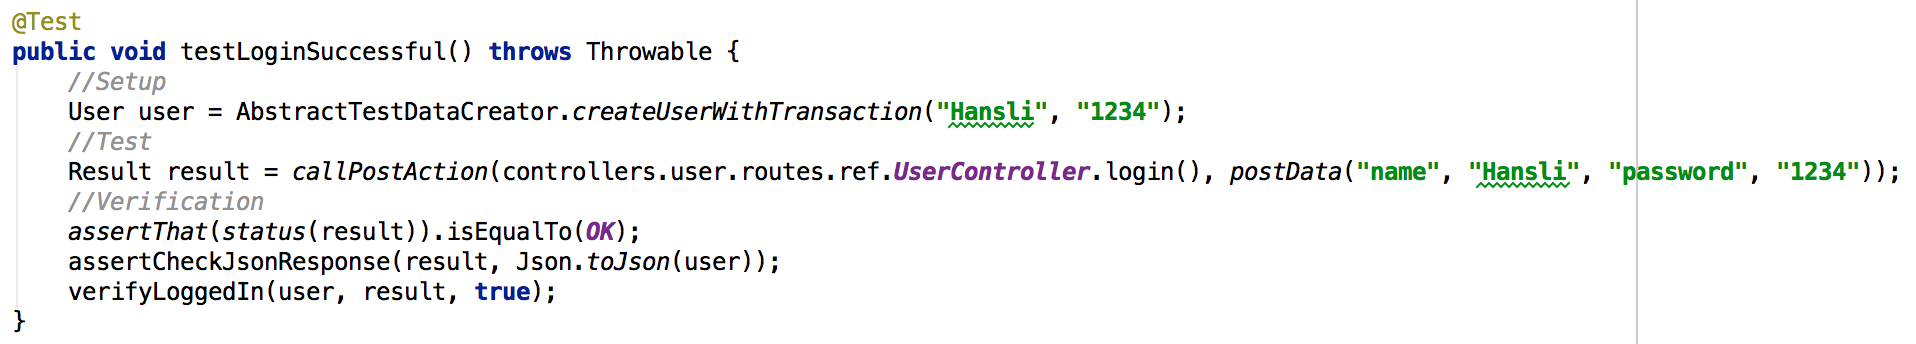
\includegraphics[scale=0.5]{projectPlan/media/img/integrationTest.png}
						\centering
						\caption{Beispiel eines Integrationstests}
						\label{fig:exampleIntegrationtest}
					\end{figure}

				\item[Behaviour (Verhaltenstests)] Gross-Integrationstests, 
					die über alle Tiers und Layers laufen. 
					Diese Tests testen Workflows von der Persistenz 
					bis zur grafischen Ausgabe im Userinterface. 
					Dazu wird mit Selenium ein Browser gestartet und dessen Ausgabe analysiert.
					In \eeppi\ sind alle Haupt-Userstories mit einem Selenium-Test abgedeckt.
					
					\begin{figure}[H]
						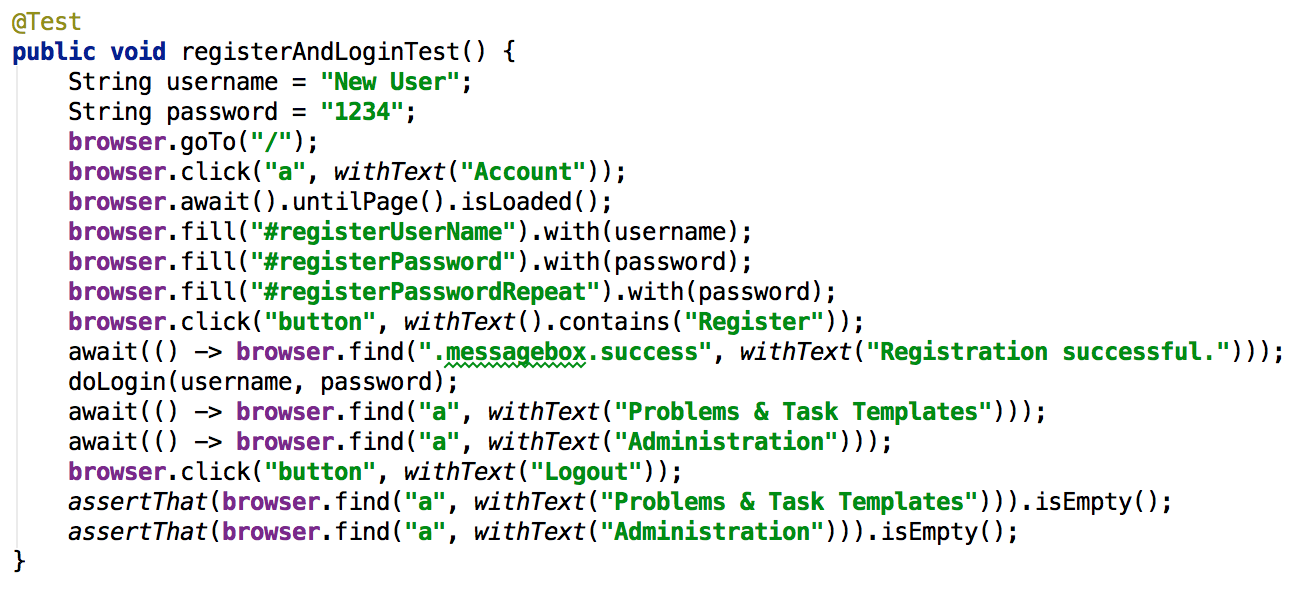
\includegraphics[scale=0.5]{projectPlan/media/img/behaviourTest.png}
						\centering
						\caption{Beispiel eines Behaviourtests (Selenium)}
						\label{fig:exampleBehaviourtest}
					\end{figure}

					Um die Schnittstellen zusammen mit den echten Systemen zu testen,
					werden die externen Systeme mit einer Vagrant-Umgebung (siehe auch Abschnitt~\ref{subsec:vagrant}) gestartet.
					Konkret läuft ein Test nach folgendem Muster ab:
					\begin{enumerate}
						\item Erstellen und starten aller benötigten Vagrant Systeme
						\item Durchführen der Tests
						\item Löschen der gestarteten Vagrant Systeme
					\end{enumerate}


			\end{description}
		
		\section{Testergebnisse}
			Die Tests wurden automatisch auf dem Jenkins (siehe Abschnitt~\ref{subsec:buildserver}) ausgeführt,
			wann immer neuer Code committed wurde.

			\begin{figure}[H]
				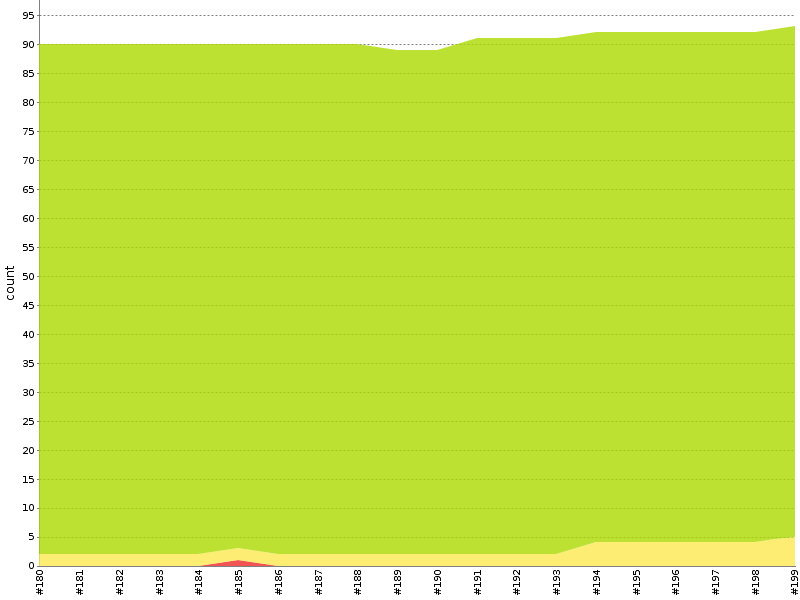
\includegraphics[width=\linewidth]{projectPlan/media/img/jenkinsTrend.png}
				\centering
				\caption{Trend der Testergebnisse auf dem Jenkins}
				\label{fig:jenkinsTrend}
			\end{figure}
			
			Einer der dabei laufenden Tests ist ein Selenium-Test, der die Client-Tests ausführt.
			Eine erfolgreiche Ausführung dieser ist in Abbildung~\ref{fig:clientTestResult} gezeigt.
			Total hat \eeppi\ rund 150 Tests, davon testen rund 1/3 den Client, knapp 2/3 den Server
			und rund 10 Tests übergeordnete Funktionalitäten und das Zusammenspiel zwischen Client und Server.
			
			\begin{figure}[H]
				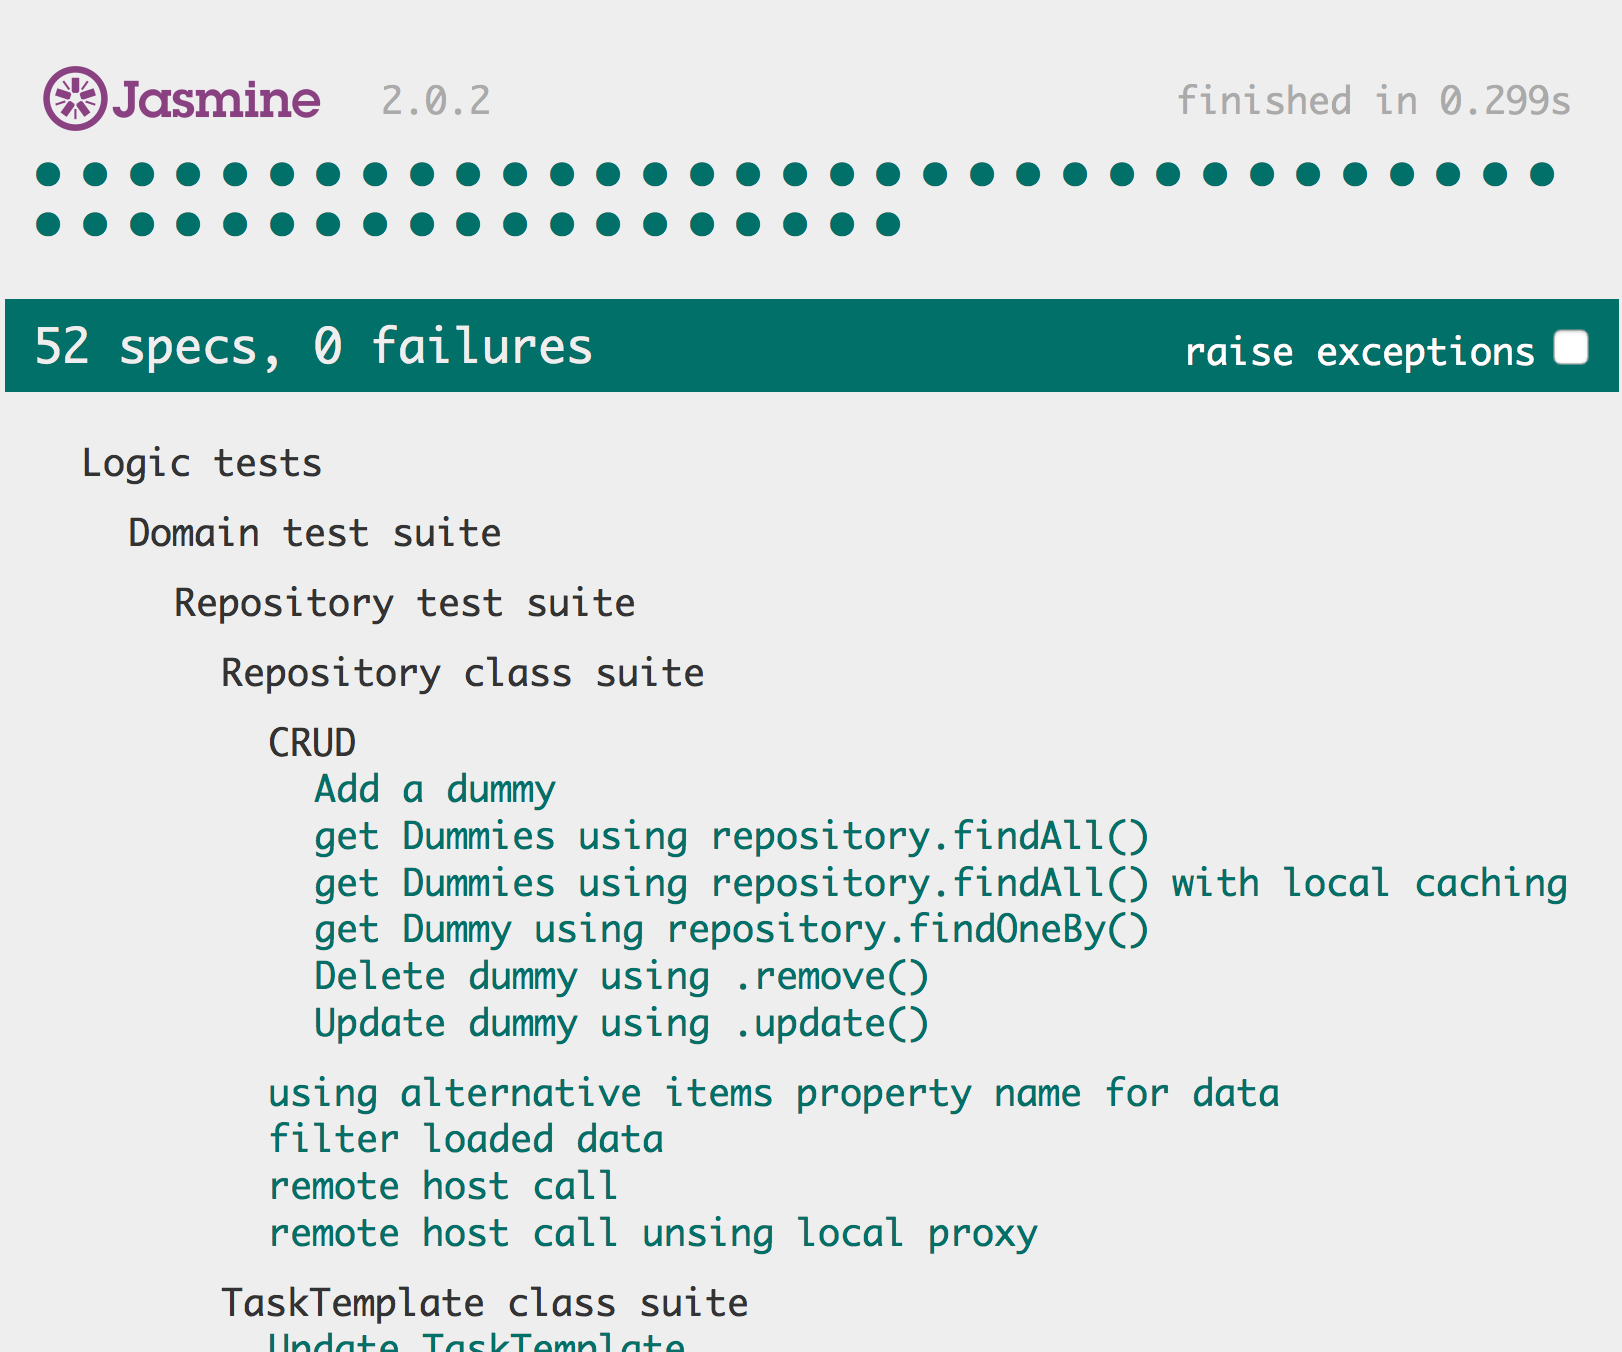
\includegraphics[width=0.8\linewidth]{projectPlan/media/img/clientTestResult.png}
				\centering
				\caption{Ergebnisse Client-Tests}
				\label{fig:clientTestResult}
			\end{figure}
